\documentclass[11pt,letterpaper,boxed]{hmcpset}
\usepackage{fullpage}
\setlength{\parskip}{6pt}
\setlength{\parindent}{0pt}
\usepackage[margin=1in]{geometry}
\usepackage{graphicx}
\usepackage{enumerate}
\usepackage{marvosym}
\usepackage{amssymb}
\usepackage{wasysym}
\usepackage{gensymb}
\usepackage{mathrsfs}
\usepackage{scrextend}
\usepackage{mathtools}
\usepackage{pgfplots}
\usepackage{xspace}
\usepackage{esvect}
\usepackage{lipsum}
\usepackage{float}
\usepackage{esint}
\usepackage{graphicx}

\name{Name $\rule{4cm}{0.15mm}$}
\class{Physics 51M Section $\rule{.5cm}{0.15mm}$ Box \# $\rule{1cm}{0.15mm}$}
\assignment{Problem Set 11}
\duedate{9 December 2019}

\begin{document}
	
	%\begin{center}
	\noindent\textbf{Collaborators:} 
	%\end{center} 
	
	%\problemlist{}
	
	\begin{problem} [HRK E6.44] In the circuit shown in Fig 36-22, the switch has been in position $a$ for a long time. It is now thrown to $b$. (a) Calculate the frequency of the resulting oscillating current. (b) What will be the amplitude of the current oscillations?
	\begin{center}
	    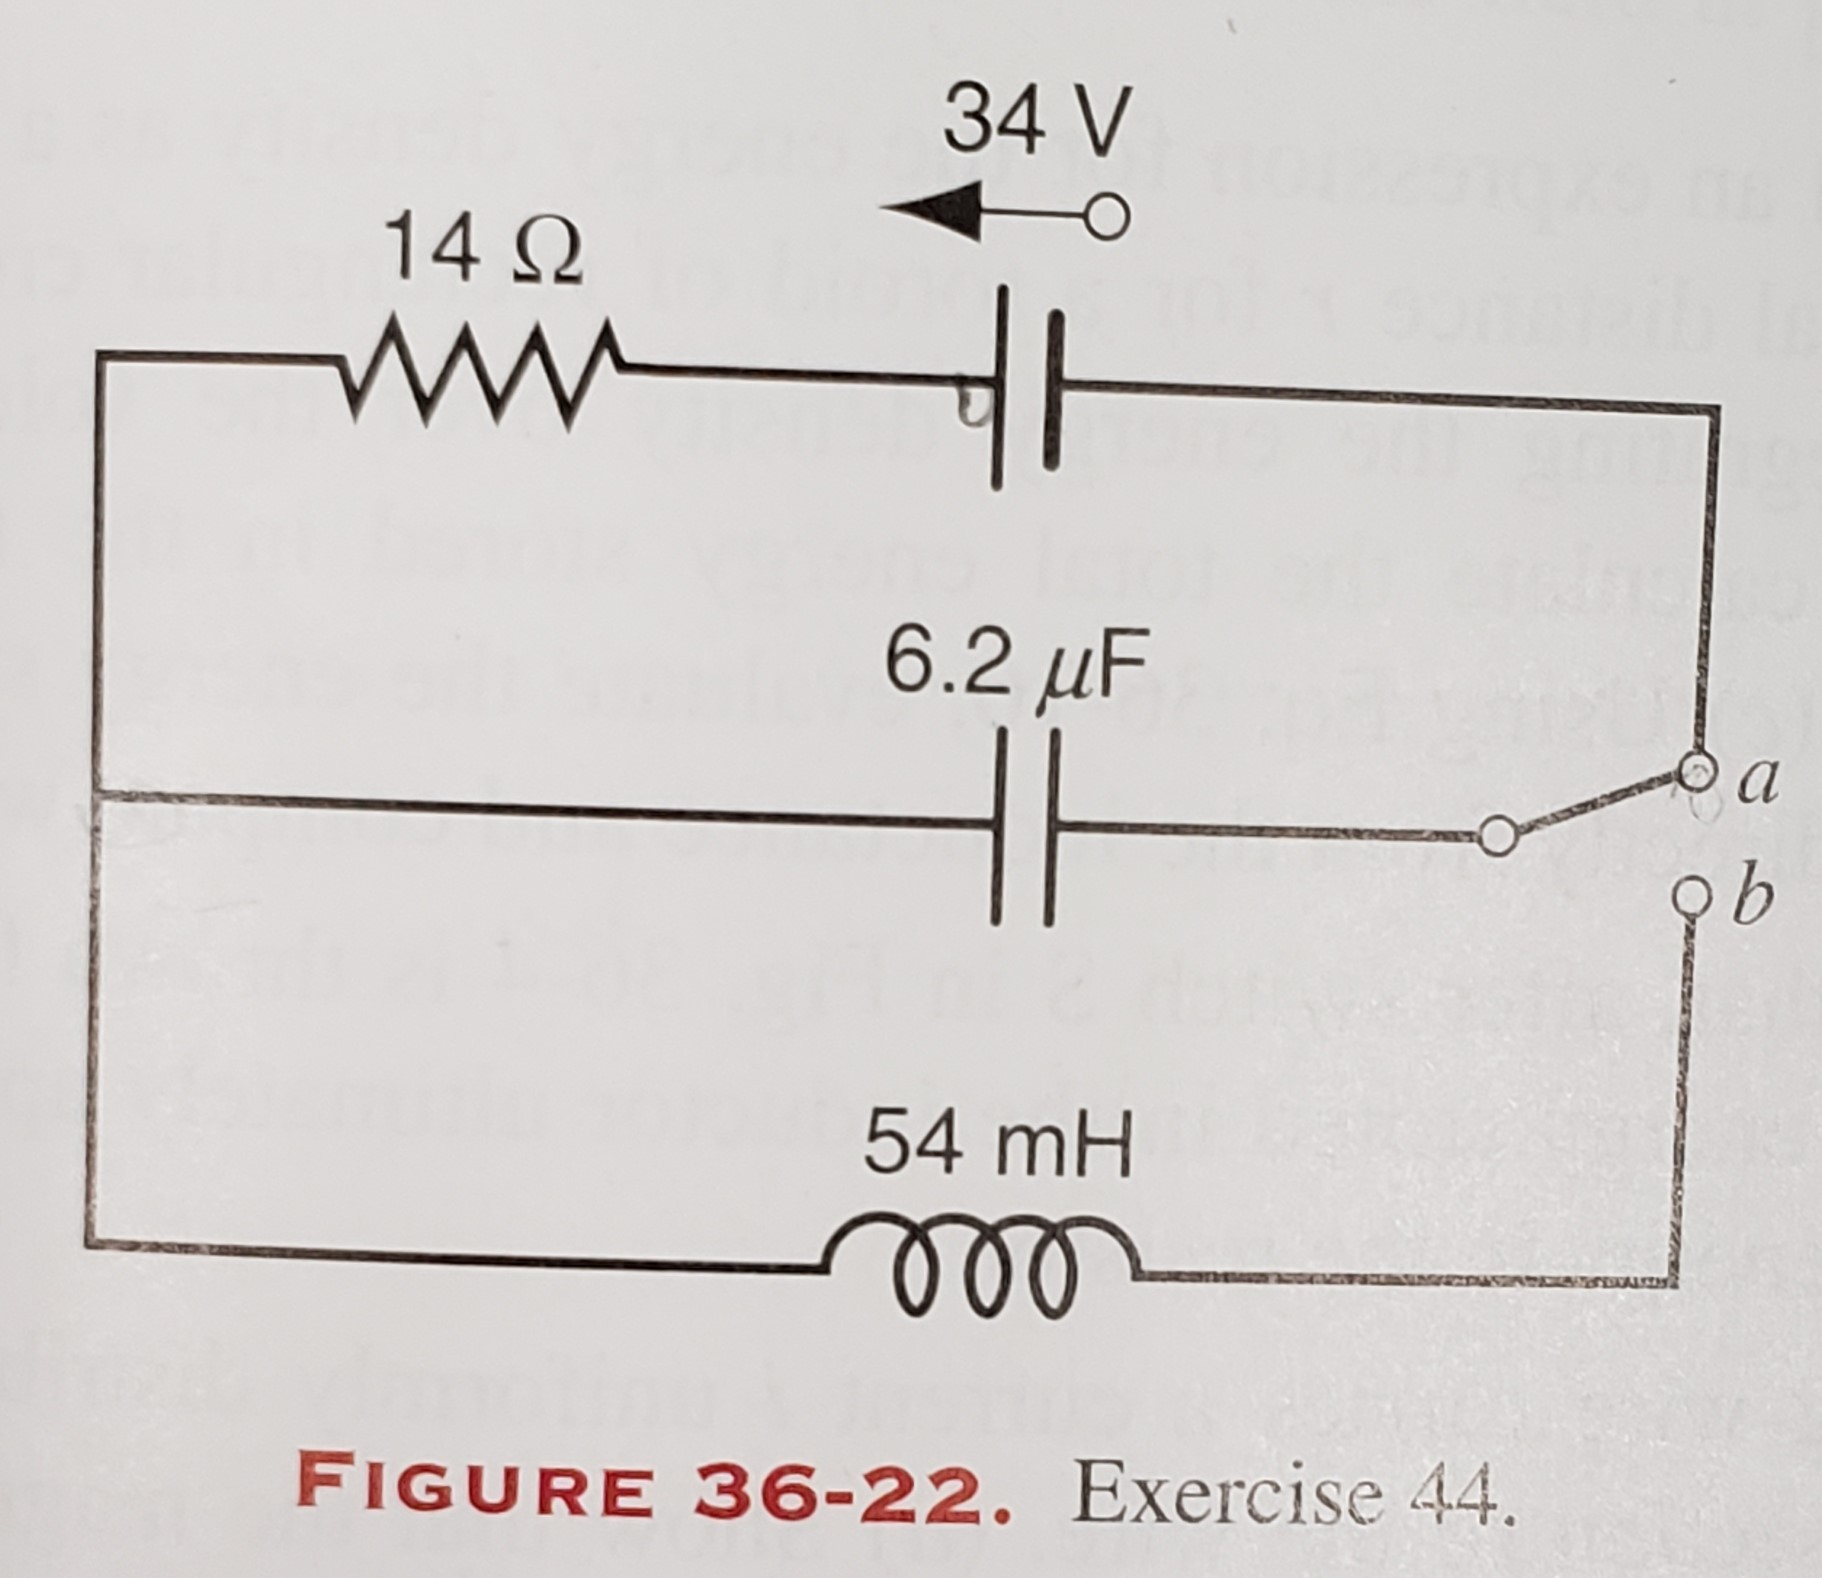
\includegraphics[scale=.075]{20191206_143722.jpg}
	    
	\end{center}
		
	\end{problem}
	
	\begin{solution}
		\vfill
	\end{solution}
	\newpage

	\begin{problem} *[HRK E34.26] A stiff wire bent into a semicircle of radius $a$ is rotated with a frequency $f$ in a uniform magnetic field, as suggested in Fig. 34-51. What are $(a)$ the frequency and $(b)$ the amplitude of the emf induced in the loop?
	\begin{center}
	    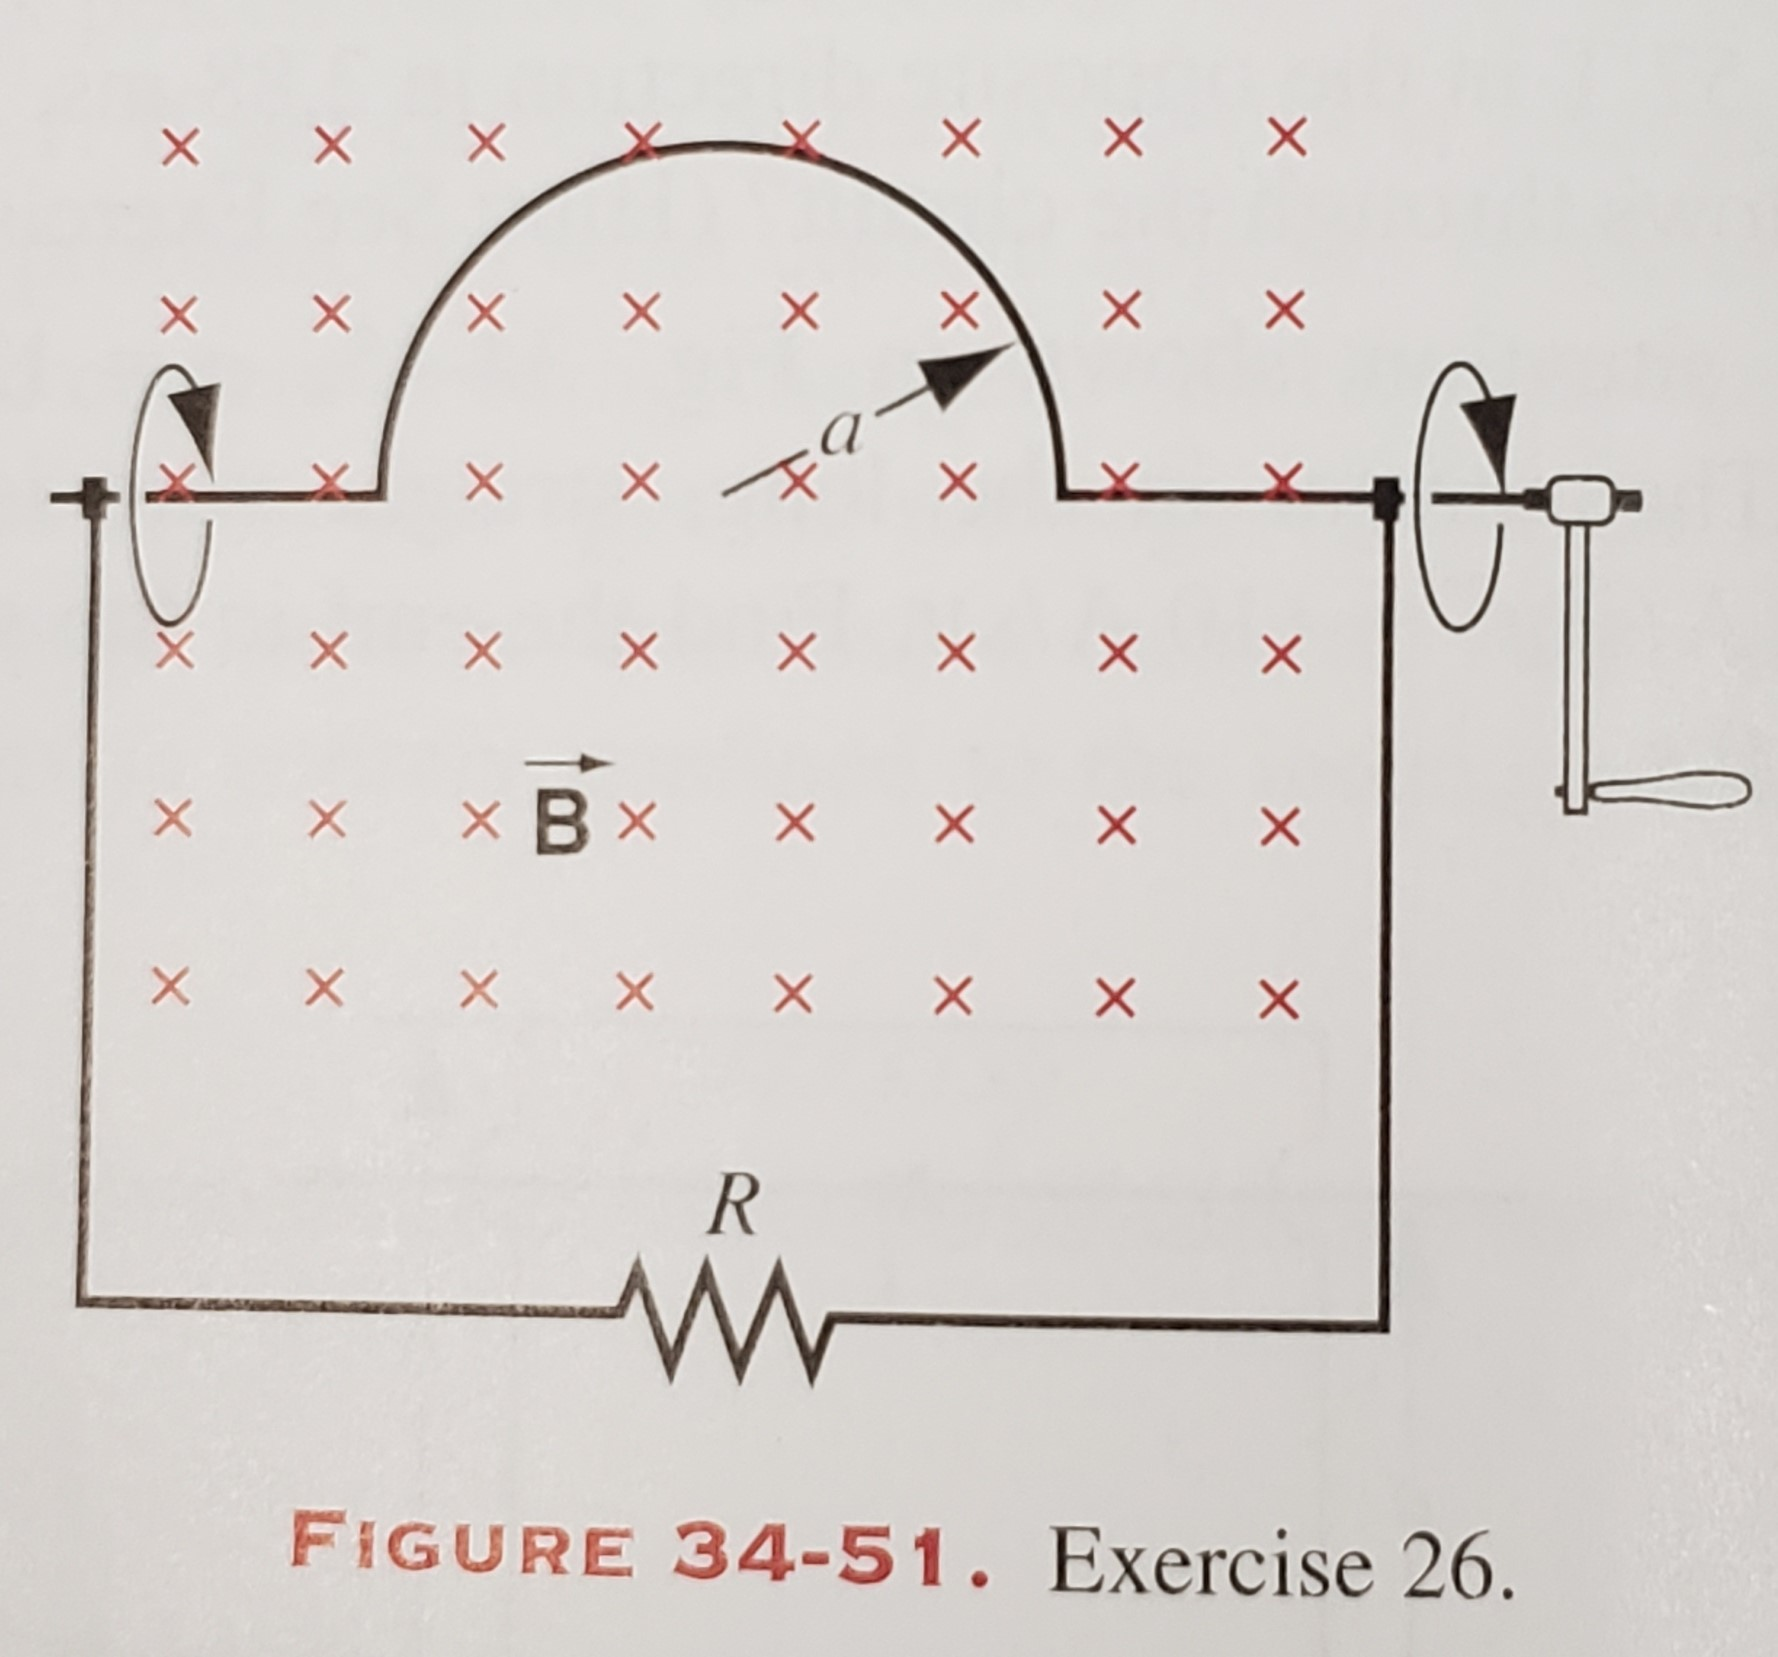
\includegraphics[scale = .075]{20191206_143753.jpg}
	\end{center}
	\end{problem}
	\begin{solution}
		\vfill
	\end{solution}
	\newpage
	
\begin{problem} [HRK P38.4] A long, cylindrical conducting rod with radius $R$ is centered on the $x$ axis as shown in Fig. 38-26. A narrow saw cut is made in the rod at $x=b$. A conduction current $i$, increasing with time and given by $i = \alpha t $, flows toward the right in the rod; $\alpha$ is a (positive) proportionality constant. At $t = 0$, there is no charge on the cut faces near $x=b$. (a) Find the magnitude of the charge on these faces, as a function of time. (b) Use Eq. 1 in Table 38-1 to find $E$ in the gap as a function of time. (c) Sketch the lines of $\vec{B}$ for $r < R$, where $r$ is the distance from the $x$ axis. (d) Use Eq. IV in Table 38-1 to find $B(r)$ in the gap for $r < R$. (e) Compare the above answer with $B(r)$ in the rod for $r < R$.
\begin{center}
    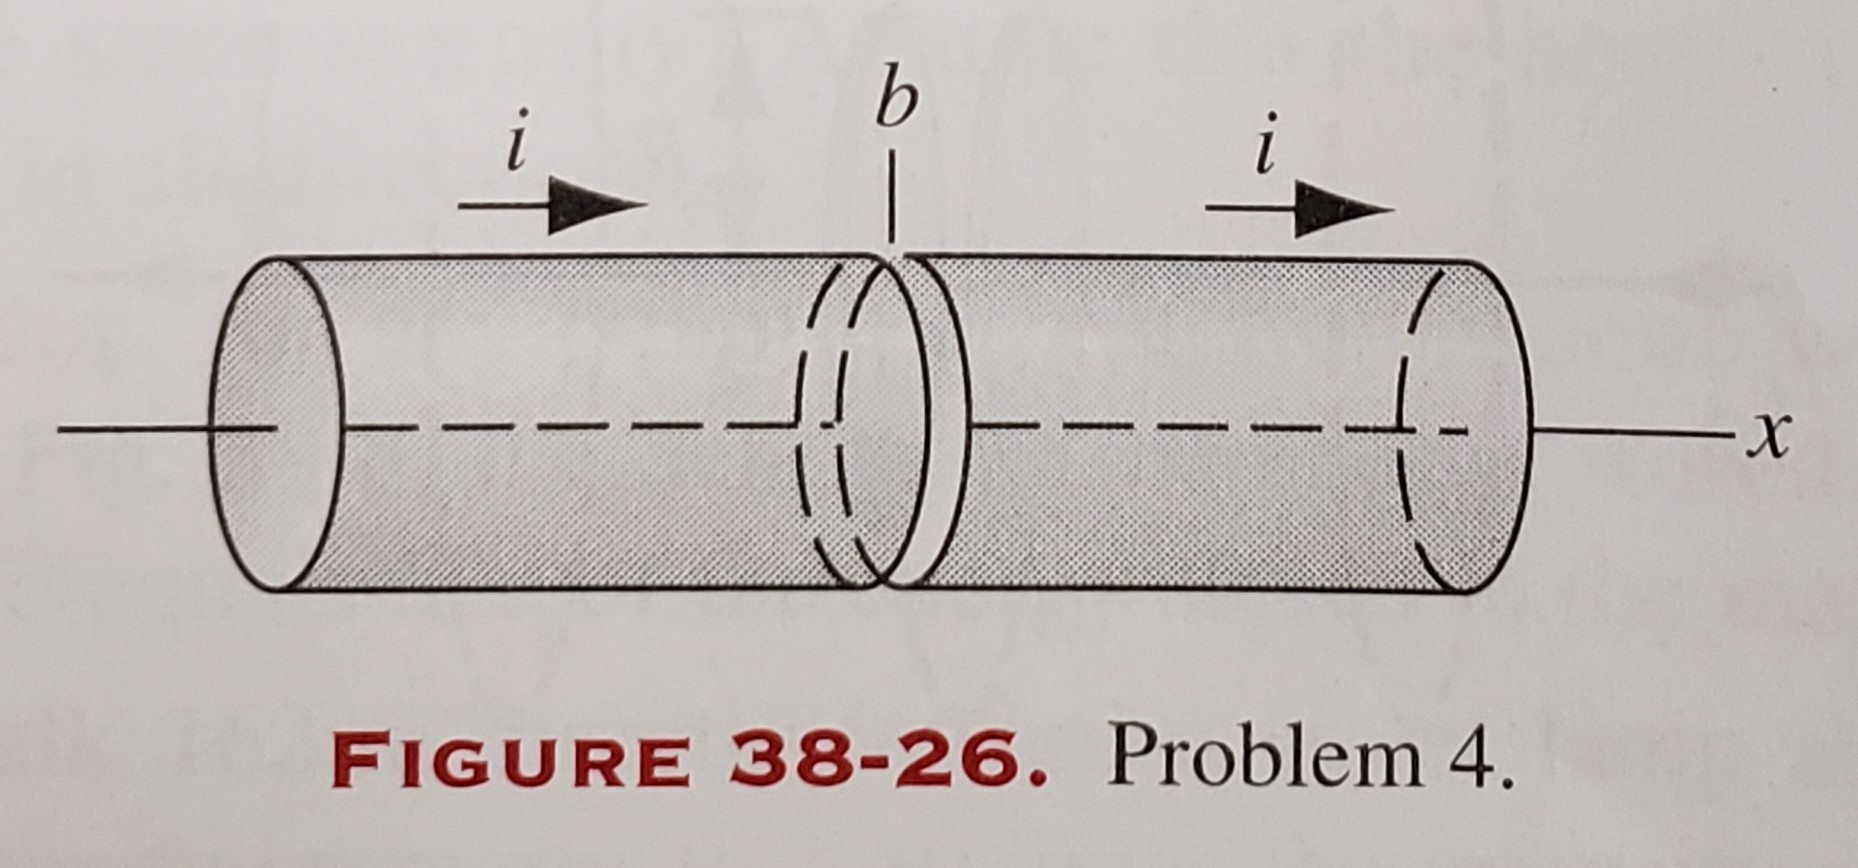
\includegraphics[scale = .075]{20191206_143840.jpg}
\end{center}
	\end{problem}
	\begin{solution}
		\vfill
	\end{solution}
	\newpage
	
\begin{problem} A parallel plate capacitor has circular plates of radius $R$ and separation $d$. The capacitor is
connected to a battery of voltage $V$ and then disconnected so that the charge ought to remain
constant. The air is humid, however, and therefore slightly conducting; thus the stored charge
leaks back across the air gap between the capacitor plates at rate $i_{leak}$. Assume that this leakage
current is uniformly distributed across the area of the plates. Find the magnetic field everywhere
between the plates.
	\end{problem}
	\begin{solution}
		\vfill
	\end{solution}
	\newpage
	
\begin{problem} In lecture we derived the wave equation for $\vec{E}$ using Maxwell’s equations in free space. Use a
similar procedure to derive a wave equation for $\vec{B}$. Show that Maxwell’s equations require that $\vec{B}$ must be transverse to the direction of propagation. (You may want to remember the vector
calculus identity $\vec{\nabla} \times (\vec{\nabla} \times \vec{C}) = \vec{\nabla} (\vec{\nabla} \cdot \vec{C}) - \nabla^2 \vec{C}$ for any $\vec{C}$.)
	\end{problem}
	\begin{solution}
		\vfill
	\end{solution}
	\newpage
	
\begin{problem} [HRK E38.16] The electric field associated with a pane electromagnetic wave is given by $E_x = 0, E_y = 0, E_z = E_0 sin k(x - ct)$, where $E_0 = 2.34 \times 10^{-4}$ V/m and $k .= 9.72 \times 10^6$ $m^{-1}$. The wave is propagating in the $+x$ direction. (a) Write expressions for the components of the magnetic field of the wave. (b) Find the wavelength of the wave.
	\end{problem}
	\begin{solution}
		\vfill
	\end{solution}
	\newpage
	
\begin{problem}  (a) Consider an electromagnetic wave in a vacuum with electric field $\vec{E} = E_0 \hat{y} sin(kx - \omega t)$.
What is the propagation direction of this electromagnetic wave?
(b) Consider an electromagnetic wave with electric field $\vec{E} = E_0 (\hat{-z}) sin(ky + \omega t)$. What is the
propagation direction of this electromagnetic wave?
(c) Consider the electric field $\vec{E} = E_0 \hat{y} [sin(kx - \omega t) + sin(kx + \omega t)]$. Show that this electric field
satisfies the wave equation $\frac{\partial^2 \vec{E}}{\partial x^2} + \frac{\partial^2 \vec{E}}{\partial y^2} + \frac{\partial^2 \vec{E}}{\partial z^2} = \frac{1}{c^2} \frac{\partial^2 \vec{E}}{\partial t^2}$

provided $\frac{\omega}{k} = c$.
	\end{problem}
	\begin{solution}
		\vfill
	\end{solution}
	\newpage
	
\end{document}